% Quadrupole mass filtering in MScan. Build from the repository root:
%   python3 docs/src/mscan_quadrupole_figures.py
%   cd docs/src && SOURCE_DATE_EPOCH=0 pdflatex -output-directory <tmp> mscan_quadrupole.tex (twice)
%   copy <tmp>/mscan_quadrupole.pdf to docs/
\pdfinfoomitdate=1
\pdftrailerid{}
\documentclass[10pt,a4paper]{article}
\usepackage[T1]{fontenc}
\usepackage{newtxtext,newtxmath}
\usepackage[margin=20mm]{geometry}
\usepackage{microtype,amsmath,booktabs,tabularx,graphicx,enumitem,xcolor}
\usepackage[font=small,labelfont=bf]{caption}
\usepackage[hidelinks]{hyperref}
\usepackage{siunitx}
\sisetup{group-separator={\,}}
\setlist{nosep,leftmargin=*}
\setlength{\parskip}{3pt}
\setlength{\parindent}{0pt}
\newcommand{\setting}[1]{\textsf{#1}}

\title{\vspace{-8mm}Quadrupole mass filtering in MScan\\[2pt]
\large Rod voltages, scan law and parameters}
\author{ESIBD Explorer Plugins, v0.5.9}
\date{November 2026}

\begin{document}
\maketitle
\vspace{-6mm}

\section{Scope}
MScan sweeps the RF amplitude $A$ of one AMX output (CH0-CH1 or CH2-CH3) and, optionally, the DC of
the two rod pairs through two AMPR channels. At each amplitude it averages the current of every
enabled DMMR module, the ion collector among them, and saves current versus $A$ for each. It does not change the AMX frequency, duty
cycle or routing. The file keeps $A$ as the axis; $m/z$ is derived from it with the settings of the
scan (Section~\ref{sec:physics}) and saved apart, as \texttt{Validation/mz}.

\section{Rod potentials}
The PSU rails of the selected AMX output are set to $V_\text{pos}=+A$ and $V_\text{neg}=-A$; the AMX
switches each rod pair between them in opposite phase, so with $s(t)=\pm1$ a square wave of 50\,\%
duty at the AMX frequency $f=\Omega/2\pi$:
\begin{align}
  \Phi_1(t) &= x + U + A\,s(t) && \text{pair 1 (AMPR channel \setting{Rod pair 1})}\\
  \Phi_2(t) &= x - U - A\,s(t) && \text{pair 2 (AMPR channel \setting{Rod pair 2})}
\end{align}
These are equations (1) and (2) of Steel and Henchman~\cite{steel} ($V_{2,4}=+U+V_0\cos\omega t$,
$V_{1,3}=-U-V_0\cos\omega t$) with $V_0=A$, the cosine replaced by $s(t)$, and a common potential $x$ (the axis).
Adding $x$ to all four rods does not change the filter: it sets the potential of the axis, hence the
axial energy of the ions. Which pair receives $+U$ does not matter either: with 50\,\% duty, swapping
the pairs only shifts the wave by half a period. Figure~\ref{fig:wave} shows an example.

\begin{figure}[h]
  \centering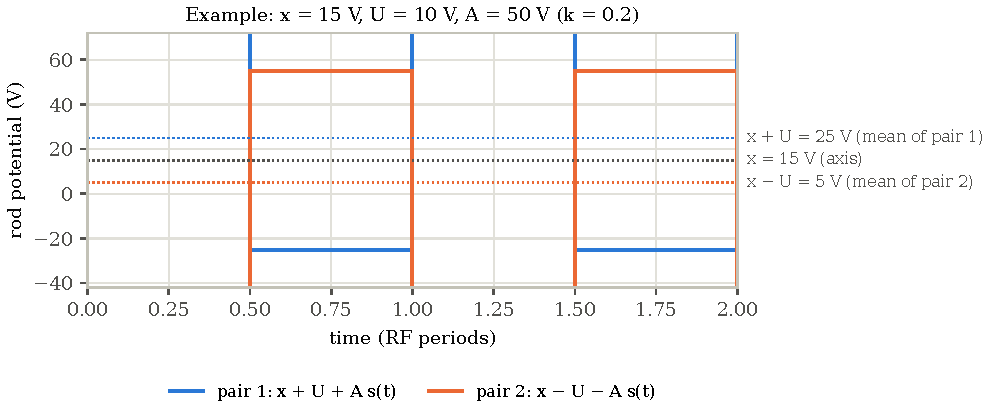
\includegraphics[width=0.92\linewidth]{mscan_quadrupole_waveforms.pdf}
  \caption{Rod potentials at one scan point. Only the antisymmetric part ($\pm U$, $\pm A\,s$) filters
  masses; $x$ is common to both pairs.}
  \label{fig:wave}
\end{figure}

\textbf{Assumptions not yet verified on the instrument.} (i) Each rod swings between $+A$ and $-A$
around its DC, i.e.\ $V_0=A$ (the AMX switches between the PSU rails, referenced to the DC applied to
that pair). (ii) The AMPR DC reaches the rods of the pair driven by the same AMX connector. (iii) The
wave on the rods stays square. A scope on the rods (or on the AMX \emph{Monitor} outputs, 1:100, if the
AMX HD has them as the 4ED does) settles all three. The lab scan of 2026-11-02 14:34 supports (ii): the
collector current responds to the difference between the two DC values and peaks when they are equal.

\section{DC law and parameters}
For a coefficient $k>0$, MScan commands at every amplitude
\begin{equation}
  U(A) = \max\bigl(U_0,\; k\,A - \delta\bigr), \qquad \Phi_{1,2}^\text{DC} = x \pm U(A).
  \label{eq:law}
\end{equation}
$k=0$ is RF-only: both pairs stay at $x$, without the floor $U_0$. A negative $k$ swaps the pairs
($U$ is computed with $|k|$). With $\delta=0$ and $k\,A\ge U_0$, equation~\eqref{eq:law} is the scan
line of the textbook~\cite{steel}: $U/A=k$ constant, a straight line through the origin.

\begin{table}[h]
\centering\small
\begin{tabularx}{\linewidth}{@{}l l l l X@{}}
\toprule
Symbol & MScan setting & Unit & Default & Role\\
\midrule
$A$ & \setting{Amplitude from / to / step} & V & -- & scanned RF amplitude, per rod (rails $\pm A$)\\
$x$ & \setting{Axis potential x} & V & 0 & common potential of the four rods, i.e.\ the axis; sets the
ion energy, does not filter. Keep the value the rods hold outside a scan.\\
$k$ & \setting{U/V ratio k} & -- & 0.2 & slope $U/A$ of the scan line; sets the resolution.
$0$ = RF-only, negative swaps the pairs.\\
$\delta$ & \setting{Resolution $\delta$} & V & 0 & lowers the line: $U/A=k-\delta/A$ rises with
$A$, so peaks keep about the same width in $A$ (Section~\ref{sec:delta}). Must be $\ge0$.\\
$U_0$ & \setting{Minimum U} & V & 0.5 & floor of $U$, must be $>0$ (Section~\ref{sec:floor}).\\
-- & \setting{Rod pair 1 / Rod pair 2} & -- & None & AMPR channels of the two pairs.
Pair 2 alone is refused.\\
\bottomrule
\end{tabularx}
\caption{Parameters of the DC law, in the \setting{Mass filter} group of the MScan panel, which also
shows a \setting{Preview} of $U$ and of both pair potentials over the scan. Settings files and HDF5
scans keep the earlier keys: \setting{Fixed offset} ($x$), \setting{Offset coefficient} ($k$),
\setting{Resolution offset} ($\delta$), \setting{Quadrupole offset} and \setting{Quadrupole offset pair 2}.}
\end{table}

\textbf{Do not confuse $k$ with the $\alpha$ of Steel and Henchman.} Their $\alpha$ is the Mathieu
parameter $a=8eU/(m r_0^2\Omega^2)$; the ratio they keep constant is $U/V_0=\alpha/(2q)=0.165$ for a
cosine. Here $k=a/(2q)$, and its useful values are near 0.2 because the wave is square
(Section~\ref{sec:physics}). Entering 0.233 as $k$ would put the line above the apex: nothing passes.

\textbf{One pair only.} If only pair 1 is selected, pair 2 keeps its own value $V_2$. The filtering DC
is then $(x+U-V_2)/2$ and the axis moves to $(x+U+V_2)/2$ during the scan. Use both pairs for
equation~\eqref{eq:law}.

\textbf{At each point.} The rails are commanded first, then both rod pairs (rounded to the AMPR display
precision). No current is acquired until the AMPR confirms each target by its setpoint readback and its
Monitor is within \setting{Voltage tolerance}. Start is refused if a value is not finite, $\delta<0$,
$U_0\le0$, a target over the span leaves the channel Min/Max or AMPR rating, or a channel is OFF or
under equation control. Normal completion restores the initial pair potentials with the PSU setpoints;
Stop or an error holds the last values.

\textbf{Recorded.} The setup keeps \texttt{offset} = \{\texttt{coefficient}, \texttt{fixed\_v},
\texttt{resolution\_offset\_v}, \texttt{minimum\_u\_v}, \texttt{pairs} (channel, AMPR module and
channel, sign, initial value)\}; every point keeps the commanded pair potentials \texttt{offset\_target} and
their Monitors \texttt{offset\_v}, one column per pair, next to \texttt{rail\_v}, \texttt{rail\_i},
sample counts and point status.

\section{What the parameters do}\label{sec:physics}
With the conventions of~\cite{steel} ($U$ and $V_0=A$ per rod, from the axis),
\begin{equation}
  a=\frac{8eU}{m r_0^2\Omega^2},\qquad q=\frac{4eA}{m r_0^2\Omega^2},\qquad \frac{a}{q}=2\,\frac{U}{A}=2k
  \quad(\delta=0).
\end{equation}
All ions lie on the line $a=2kq$; an ion passes when its point is inside the stability region
(Figure~\ref{fig:stab}). For a 50\,\% square wave the apex is at $a=0.2381$, $q=0.5529$, i.e.\
$k=0.2153$ (cosine: 0.2370, 0.7060, $k=0.1678$). The RF-only limit is $q=0.712$ (cosine 0.908).

\begin{figure}[h]
  \centering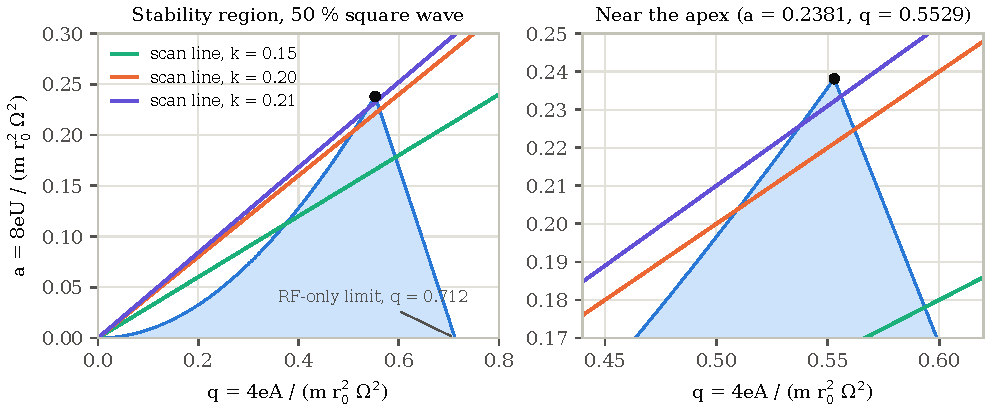
\includegraphics[width=0.98\linewidth]{mscan_quadrupole_stability.pdf}
  \caption{Stability region of the 50\,\% square wave (both directions stable) and scan lines
  $a=2kq$. Computed with the transfer matrix of the piecewise-constant Hill equation.}
  \label{fig:stab}
\end{figure}

\begin{table}[h]
\centering\small
\begin{tabular}{@{}cccc@{}}
\toprule
$k$ & transmitted $q$ band & centre $\bar q$ & $R=\bar q/\Delta q$\\
\midrule
0 & 0 -- 0.712 & -- & high-pass\\
0.10 & 0.246 -- 0.629 & 0.438 & 1.1\\
0.15 & 0.375 -- 0.593 & 0.484 & 2.2\\
0.18 & 0.455 -- 0.574 & 0.515 & 4.3\\
0.19 & 0.482 -- 0.568 & 0.525 & 6.1\\
0.20 & 0.510 -- 0.562 & 0.536 & 10.3\\
0.205 & 0.524 -- 0.559 & 0.542 & 15.4\\
0.21 & 0.538 -- 0.556 & 0.547 & 30.4\\
0.2125 & 0.545 -- 0.554 & 0.550 & 57\\
\bottomrule
\end{tabular}
\caption{Transmitted $q$ band versus $k$ ($\delta=0$, ideal 50\,\% square wave). Near the apex
$R\approx0.157/(0.2153-k)$. $R$ is $m/\Delta m$ of the band at fixed $A$.}
\label{tab:band}
\end{table}

\textbf{Peak position.} An ion transmitted at the centre $\bar q$ of the band has
\begin{equation}
  \frac{m}{z}\,[\mathrm{Th}] \approx 2.444\,\frac{A\,[\mathrm V]}{\bar q}
  \left(\frac{4\,\mathrm{mm}}{r_0}\right)^{\!2}\left(\frac{500\,\mathrm{kHz}}{f}\right)^{\!2},
\end{equation}
about $4.56\,A$ at $k=0.2$ for $r_0=4$\,mm and 500\,kHz. MScan computes it at every point, with
$\bar q$ from $U/V_0$ there, the AMX frequency, \setting{r0} and the \setting{RF attenuation factor}
$c=V_0/A$, shows it as \setting{m/z range} and on the plot (\setting{Plot axis}), and saves it as
\texttt{Validation/mz}. On 2026-11-03 the Agilent G2421A tuning mix gave its ions 622, 922, 1522 and
2122 on Q2 at 400, 450 and 500\,kHz: $c=0.978$ (band widths at $k=0.20$, transmission at $k=0.21$)
and an effective $r_0=2.625$\,mm, now the defaults: 5\,\% above the nominal 2.5\,mm of Q2 (5\,mm
between opposite rods), about 10\,\% in $m/z$. The filter then closes at $k=0.2153\,c=0.2105$. In RF-only mode ($k=0$) ions with
$m/z<3.43\,A$ (same units) are rejected, so a spectrum of several species is a staircase: each species
removes a step at its cut-off amplitude $A_c$, and its peak at $k=0.2$ lies near $0.753\,A_c$.
The mass window scales as $A/f^2$: at fixed $A_\text{max}$, 300\,kHz reaches 2.8 times and 200\,kHz
6.3 times the $m/z$ of 500\,kHz. The rail current also scales with $f$ (Section~\ref{sec:limits}).

\textbf{Resolution and the amplitude on the rods.} Table~\ref{tab:band} assumes $V_0=A$. If the rods
see $cA$, the filter works at $k/c$: at $k=0.20$ it closes completely for $c<0.929$, at $k=0.21$ for
$c<0.975$. The scan itself measures $c$: raise $k$ until the signal disappears at $k_c$; then
$c=k_c/0.2153$. Rounded edges matter much less: a trapezoid with rise times of 100, 200, 300 and
500\,ns at 500\,kHz moves the apex to $k=0.2141$, 0.2111, 0.2064 and 0.1921; an exponential edge
with $\tau=50$, 100, 150\,ns to 0.2123, 0.2044, 0.1937. With DC coupling, a duty error of 1\,\% moves
the apex by about $\pm0.018$ in $k$.

\textbf{Resolution $\delta$.}\label{sec:delta} With $\delta=0$ the peak width grows in
proportion to $A$ (constant $R$). With $k$ at the apex value and $U=kA-\delta$, the width is nearly
constant, $\Delta A\approx6.4\,\delta$ (simulated: 6.8, 6.5, 6.4, 6.4\,V at $A=50$, 100, 200, 300\,V
for $\delta=1$\,V). Commercial instruments set slope and intercept on a light and a heavy reference
ion, because the ideal constant-width line is a curve~\cite{pedder}. A negative $\delta$ (a positive
constant added to $kA$) at the apex slope passes nothing, which is why MScan refuses $\delta<0$.

\textbf{Minimum U.}\label{sec:floor} At zero DC every ion heavier than the RF-only cut-off passes.
Without a floor, a scan starting near $A=0$ begins with an unfiltered plateau (simulated for an ion
with its peak at 300\,V and $\delta=1$\,V: transmitted from 0 to 4.72\,V with $\max(0,\cdot)$, only from
4.57 to 4.72\,V without clamping). Commercial residual gas analysers keep the DC from reaching zero
(``Zero Blast Suppression''~\cite{srs}). Peaks below $A^*=(U_0+\delta)/k$ are not filtered reliably.

\section{Limits of the present set-up}\label{sec:limits}
\begin{itemize}
\item Rail current of the Q2 output (AMX HD, 500\,kHz, lab 2026-11-02): about
  $\SI{12}{mA} + \SI{0.565}{mA/V}\times A$ per rail, i.e.\ \SI{153}{mA} at 250\,V. With
  $I_\text{lim}=\SI{200}{mA}$ the amplitude cannot exceed about 333\,V at 500\,kHz, even with the PSU
  range switched on. The current scales with $f$: about \SI{97}{mA} at 300\,kHz and 250\,V.
\item PSU headroom (PSU\_A in Half range, lab 2026-11-03): output + dropout fell from 256\,V at 0\,mA
  to about 248.5\,V at 150\,mA, so the rails could not regulate above about 248\,V and a 50--300\,V
  scan stopped at 250\,V. MScan now refuses a scan above output + dropout $-$ 2\,V, stops at once when
  a rail has lost its headroom, and flags points measured with less than 2\,V
  (\texttt{low\_headroom}). Full range raises the internal supply; check the dropout and the PSU
  temperature at the highest amplitude.
\item The scan law is applied by two instruments (PSU and AMPR) that must agree to better than 1\,\%
  in ratio near the apex. Rectangular-wave (digital) quadrupoles can instead keep the amplitude and
  the DC fixed and sweep the frequency: $U/A$ is then constant by construction and $m/z\propto1/f^2$.
  MScan does not do this.
\item A filter without DC is also possible with DC-coupled square waves by changing the duty cycle
  (computed: $R\approx7$ at 60.0\,\%, 12 at 60.5\,\%, 41 at 61.0\,\%; closed above about 61.2\,\%).
  MScan does not do this either; it leaves the AMX timing unchanged.
\end{itemize}

\section{Recommended order on a new set-up}
\begin{enumerate}
\item Confirm ions on the collector at a fixed amplitude: the current must be positive (for positive
  ions) and fluctuate with the spray. The electrospray current alone does not prove that ions enter.
\item Record one scan with the electrospray HV off: it gives the background of the collector, which
  MScan does not subtract.
\item Scan with $k=0$ to the highest available $A$: count the cut-off steps and note their $A_c$.
\item Scan with $k=0.15$, 0.18, 0.20, 0.21 ($\delta=0$, $U_0=0.5$\,V); the value where the signal
  vanishes gives $c$ (amplitude on the rods / $A$).
\item Only then use $\delta$, set on two reference ions, if constant peak width is needed.
\end{enumerate}

\begin{thebibliography}{9}\small
\bibitem{steel} C.~Steel, M.~Henchman, \emph{Understanding the Quadrupole Mass Filter through Computer
Simulation}, J.\ Chem.\ Educ.\ 75 (1998) 1049.
\bibitem{pedder} R.~E.~Pedder, \emph{Practical Quadrupole Theory: Graphical Theory}, Extrel
Application Note RA\_2010A (ASMS 2001).
\bibitem{srs} Stanford Research Systems, \emph{RGA120/220/320 Residual Gas Analyzer, User Manual},
rev.\ 1.08 (2025), section ``Zero Blast Suppression''.
\end{thebibliography}
\end{document}
